\documentclass[10pt,a4paper]{article}
\usepackage[margin=20mm]{geometry}
\usepackage{fontspec}
\setmainfont{Liberation Serif}
\setsansfont{Liberation Sans}
\setmonofont{Liberation Mono}[Scale=MatchLowercase]
\usepackage{amsmath,graphicx,booktabs,url,caption}
\usepackage[hidelinks]{hyperref}
\captionsetup{font=small,labelfont=bf}
\renewcommand{\thetable}{S\arabic{table}}
\renewcommand{\thefigure}{S\arabic{figure}}
\setlength{\parindent}{0pt}
\setlength{\parskip}{5pt}
\title{\vspace{-12mm}\large\bfseries Supplementary Material:\\A Scene-Aware Bidirectional Evaluation on RDD2022}
\author{\normalsize Lê Thành Luân, Phạm Bá Anh Tuấn}
\date{}
\begin{document}
\maketitle
\vspace{-8mm}
\section*{Scope and conventions}
This supplement accompanies the three-variant, 18-run evaluation. All results are calculated from the supplied archive metrics. Percentages are AP or mAP multiplied by 100; gaps are in percentage points. Uncertainty denotes sample standard deviation over seeds 13, 37, and 71. No confidence interval, additional training run, or independent inference replay is introduced. CSV files preserve unrounded values.

\section*{Complete class-level results}
Table~\ref{tab:classap} gives the four-class AP matrix. Rows sharing a target use identical test images. Means are not rankings of individual runs. YOLO26n has the highest in-domain mean mAP but does not have the highest AP for every class.

\begin{center}
\captionof{table}{Full-test AP@50:95 by class (\%, three-seed means). Class-specific SDs are retained in \texttt{data/metric\_summary.csv}.}
\label{tab:classap}
\begin{tabular}{lllrrrr}\toprule
Model & Train & Target & D00 & D10 & D20 & D40\\\midrule
YOLOv8n & Drone & Drone & 30.96 & 34.66 & 19.45 & 0.57 \\
YOLOv8n & MotorBike & Drone & 6.27 & 8.91 & 0.72 & 10.31 \\
YOLO11n & Drone & Drone & 32.45 & 36.48 & 17.42 & 3.20 \\
YOLO11n & MotorBike & Drone & 6.51 & 11.26 & 1.43 & 9.80 \\
YOLO26n & Drone & Drone & 33.37 & 39.57 & 22.94 & 2.06 \\
YOLO26n & MotorBike & Drone & 10.07 & 13.34 & 2.89 & 4.02 \\
YOLOv8n & Drone & MotorBike & 20.58 & 16.23 & 2.14 & 1.11 \\
YOLOv8n & MotorBike & MotorBike & 47.18 & 50.66 & 55.35 & 51.83 \\
YOLO11n & Drone & MotorBike & 20.98 & 17.35 & 1.00 & 1.26 \\
YOLO11n & MotorBike & MotorBike & 48.31 & 53.05 & 58.72 & 52.27 \\
YOLO26n & Drone & MotorBike & 24.27 & 22.75 & 1.54 & 1.38 \\
YOLO26n & MotorBike & MotorBike & 50.44 & 53.66 & 57.99 & 56.93 \\
\bottomrule

\end{tabular}
\end{center}

\section*{Seed consistency and complementary metric}
Each entry in Table~\ref{tab:seedgaps} subtracts the other-domain-trained score from the target-domain-trained score on identical target images for one model and seed. All 18 full-test gaps are positive. Gap SDs in the main paper are calculated from these differences before aggregation. Table~\ref{tab:map50} provides full-test mAP@50.

\noindent\begin{minipage}[t]{0.48\textwidth}
\captionof{table}{Full-test fixed-target mAP@50:95 gaps (pp) by seed.}
\label{tab:seedgaps}\centering\small
\setlength{\tabcolsep}{4pt}
\begin{tabular}{llrrr}\toprule
Model & Target & 13 & 37 & 71\\\midrule
YOLOv8n & Drone & 15.03 & 13.52 & 16.01 \\
YOLOv8n & MotorBike & 40.39 & 42.40 & 40.93 \\
YOLO11n & Drone & 16.27 & 10.84 & 18.29 \\
YOLO11n & MotorBike & 43.49 & 42.47 & 42.85 \\
YOLO26n & Drone & 16.91 & 16.10 & 17.71 \\
YOLO26n & MotorBike & 43.14 & 42.87 & 40.80 \\
\bottomrule

\end{tabular}
\end{minipage}\hfill
\begin{minipage}[t]{0.49\textwidth}
\captionof{table}{Full-test mAP@50 (\%, mean $\pm$ sample SD).}
\label{tab:map50}\centering\small
\setlength{\tabcolsep}{3pt}
\begin{tabular}{llrr}\toprule
Model & Train & Drone & MotorBike\\\midrule
YOLOv8n & Drone & $44.17\pm2.77$ & $24.29\pm3.28$ \\
YOLOv8n & MotorBike & $18.02\pm6.99$ & $84.68\pm0.13$ \\
YOLO11n & Drone & $45.51\pm3.73$ & $23.44\pm2.34$ \\
YOLO11n & MotorBike & $20.81\pm11.78$ & $84.54\pm0.31$ \\
YOLO26n & Drone & $48.73\pm2.09$ & $27.47\pm0.44$ \\
YOLO26n & MotorBike & $18.11\pm0.61$ & $86.75\pm0.74$ \\
\bottomrule

\end{tabular}
\end{minipage}

\newpage
\section*{Excluded-label sensitivity and validation dynamics}
The clean-only rule removes images with excluded-class annotations, leaving 273 Drone and 271 MotorBike images; it does not require all four target classes in each image. Table~\ref{tab:clean} reports the scores. All 18 clean-only seed gaps are positive. Mean $\pm$ SD gaps on Drone/MotorBike targets are $15.25\pm1.58$/$41.87\pm1.34$~pp for YOLOv8n, $14.93\pm4.42$/$43.86\pm0.63$~pp for YOLO11n, and $16.59\pm0.95$/$42.60\pm1.87$~pp for YOLO26n. Score changes cannot be isolated from the changed image population.

\noindent\begin{minipage}[t]{0.49\textwidth}
\captionof{table}{Clean-only mAP@50:95 (\%, mean $\pm$ sample SD).}
\label{tab:clean}\centering\small
\setlength{\tabcolsep}{3pt}
\begin{tabular}{llrr}\toprule
Model & Train & Drone & MotorBike\\\midrule
YOLOv8n & Drone & $23.03\pm1.22$ & $10.33\pm1.35$ \\
YOLOv8n & MotorBike & $7.78\pm2.73$ & $52.20\pm0.46$ \\
YOLO11n & Drone & $23.71\pm2.50$ & $10.72\pm0.58$ \\
YOLO11n & MotorBike & $8.79\pm4.05$ & $54.59\pm0.60$ \\
YOLO26n & Drone & $26.09\pm0.91$ & $13.57\pm0.12$ \\
YOLO26n & MotorBike & $9.49\pm0.47$ & $56.17\pm1.76$ \\
\bottomrule

\end{tabular}
\end{minipage}\hfill
\begin{minipage}[t]{0.48\textwidth}
\captionof{table}{Epoch of maximum logged source-validation mAP@50:95.}
\label{tab:peaks}\centering\small
\setlength{\tabcolsep}{4pt}
\begin{tabular}{llrrr}\toprule
Model & Train & Seed 13 & Seed 37 & Seed 71\\\midrule
YOLOv8n & Drone & 63 & 133 & 129 \\
YOLOv8n & MotorBike & 120 & 109 & 119 \\
YOLO11n & Drone & 110 & 92 & 111 \\
YOLO11n & MotorBike & 128 & 131 & 113 \\
YOLO26n & Drone & 117 & 81 & 119 \\
YOLO26n & MotorBike & 126 & 82 & 128 \\
\bottomrule

\end{tabular}
\end{minipage}

\vspace{4mm}
Fig.~\ref{fig:training} displays all 18 source-validation trajectories; Table~\ref{tab:peaks} records their mAP-maximum epochs. Every run completed 150 epochs with patience zero. A logged validation maximum is distinct from independently verifying the checkpoint-selection fitness. These curves contain no test-set metrics.

\begin{center}
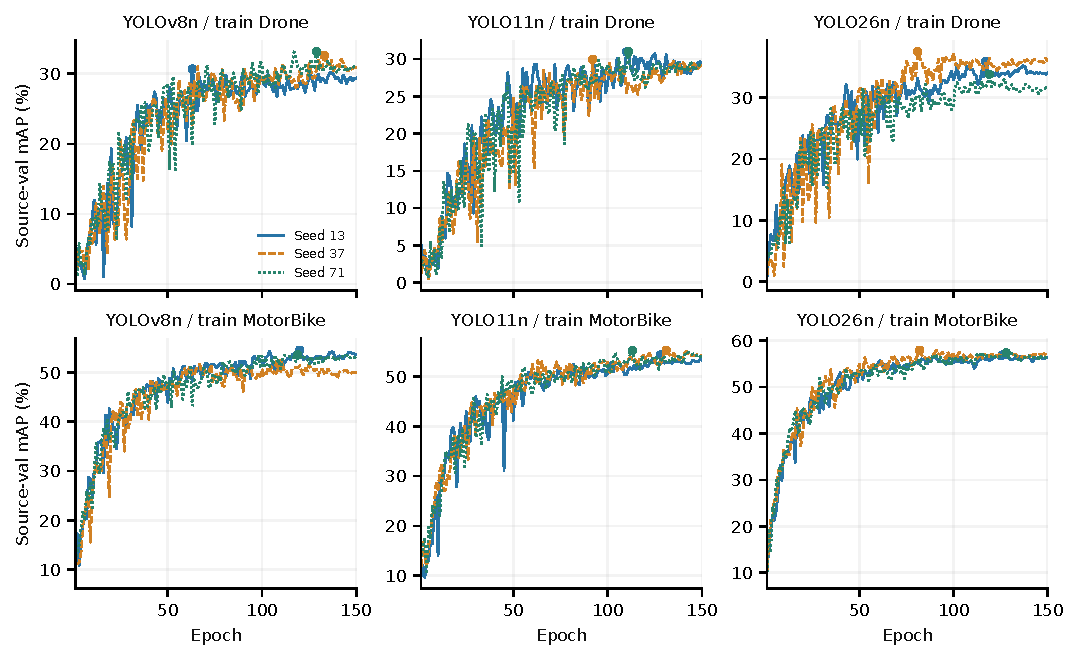
\includegraphics[width=0.95\textwidth]{figures/validation_curves_light.pdf}
\captionof{figure}{Source-validation mAP@50:95 for three YOLO variants and two training domains. Each panel contains seeds 13, 37, and 71; circles mark their maximum logged validation mAP. Line styles distinguish seeds as well as colors.}
\label{fig:training}
\end{center}

\section*{Regeneration and evidence boundary}
The package retains the 72 metric rows, run identities, 18 training-log CSVs, and summary tables. Model, training domain, target domain, seed, and subset jointly identify a metric row; \texttt{D13} alone is not unique. The supplied preparation and build scripts regenerate tables, figures, and PDFs from retained records; commands are documented in the package README. The optional white-background gap-summary figure is supplied separately, because the same numbers already appear in the main paper. Regeneration reproduces manuscript artifacts from archived summaries, not training or original-image evaluation.
\end{document}
